\section{Ablation Study}
\label{sec:ablation}

\subsection{Memory Module Ablation}
\begin{table}[t]
  \centering
  \small
  \setlength{\tabcolsep}{4pt}
  \renewcommand{\arraystretch}{1.08}
  \caption{Memory-efficient module comparison under fixed pseudo-label ablation setting. This experiment analyzes Memory Tokens and Memory Attention Time, not as full protocol main results.}
  \label{tab:memory_ablation}
  \begin{tabular}{lrrrr}
    \toprule
    Method & Memory Tokens$\downarrow$ & mIoU$\uparrow$ & BFScore$\uparrow$ & Mem. Attn. (s)$\downarrow$ \\
    \midrule
    OmniSAM & 32768 & 60.26 & 39.59 & 117.48 \\
    OmniSAM + Confidence Mask & 32768 & 60.26 & 39.59 & 117.56 \\
    OmniSAM + Confidence Mask + MTC & 8192 & 60.12 & 39.23 & 61.00 \\
    OmniSAM + Confidence Mask + SMR & 16384 & 60.09 & 39.23 & 79.69 \\
    OmniSAM + MTC+SMR & 4096 & 60.02 & 39.23 & 52.38 \\
    OmniSAM + Confidence Mask + MTC+SMR & 4096 & 60.02 & 39.23 & 51.92 \\
    \bottomrule
  \end{tabular}
\end{table}


Table~\ref{tab:memory_ablation} adopts a fixed pseudo-label ablation setting, reusing the same pseudo-labels to isolate memory module effects, not replacing the end-to-end main results in Section~\ref{sec:experiments}. OmniSAM + Confidence Mask does not reduce Memory Tokens, and its Memory Attention Time is essentially consistent with OmniSAM, indicating that only changing pseudo-label filtering without reducing attention input cannot obtain computational gains from this module. After separately enabling MTC or SMR on top of Confidence Mask, Memory Tokens and Memory Attention Time decrease synchronously, verifying that both spatial aggregation and content selection can reduce historical memory interaction. The combined configuration further compresses tokens from 32768 to 4096 and reduces attention time to 51.92s, while accompanied by slight mIoU and BFScore costs, reflecting efficiency-accuracy trade-offs.

As shown in Figure~\ref{fig:speed_accuracy_tradeoff}, memory-efficient configurations trade small accuracy changes for training efficiency gains. The points of different modules do not form a monotonic accuracy improvement relationship, further indicating that the main value of MTC and SMR is controlling training cost rather than enhancing segmentation accuracy. This figure is used for module trend analysis and is not part of full protocol main results.

\begin{figure}[t]
    \centering
    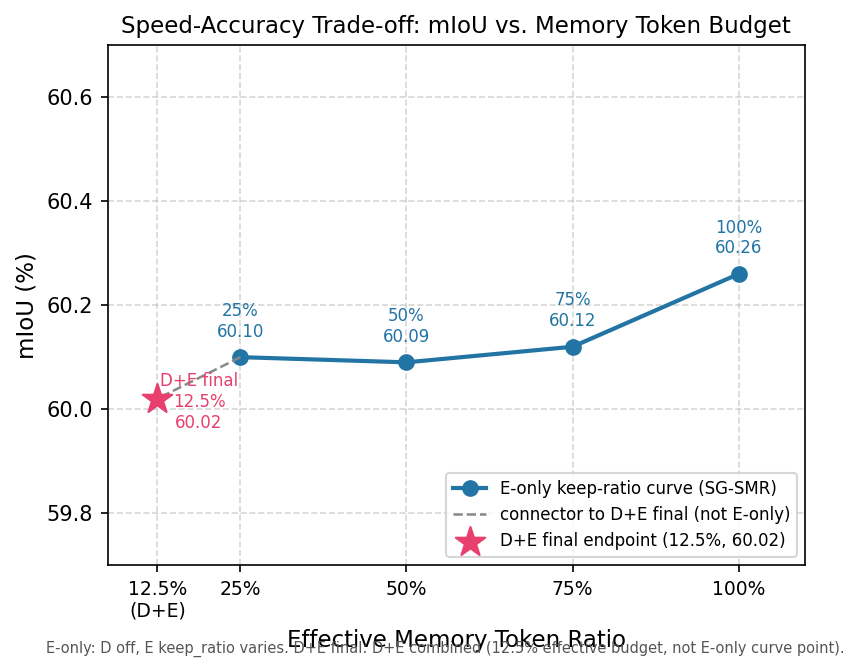
\includegraphics[width=0.78\linewidth]{figures/fig_speed_accuracy_tradeoff_miou.png}
    \caption{Training efficiency vs. mIoU trade-off under fixed pseudo-label ablation setting. Different configurations demonstrate efficiency gains from memory token reduction and corresponding accuracy changes. This figure is not part of full protocol main results.}
    \label{fig:speed_accuracy_tradeoff}
\end{figure}

\subsection{Token Budget}
\begin{table}[t]
  \centering
  \small
  \setlength{\tabcolsep}{3pt}
  \renewcommand{\arraystretch}{1.08}
  \caption{Accuracy and efficiency trade-offs under different Memory Token budgets. Results from fixed pseudo-label ablation setting.}
  \label{tab:token_budget}
  \begin{tabular}{lrrrrr}
    \toprule
    Token Budget & Tokens$\downarrow$ & mIoU$\uparrow$ & BFScore$\uparrow$ & Step (s)$\downarrow$ & Mem. Attn. (s)$\downarrow$ \\
    \midrule
    100\% & 32768 & 60.26 & 39.59 & 2.4089 & 117.56 \\
    75\% & 24576 & 60.12 & 39.28 & 2.4614 & 98.62 \\
    50\% & 16384 & 60.09 & 39.23 & 2.3798 & 79.69 \\
    25\% & 8192 & 60.10 & 39.29 & 2.2941 & 60.54 \\
    12.5\%$^{\dagger}$ & 4096 & 60.02 & 39.23 & 2.3153 & 51.92 \\
    \bottomrule
  \end{tabular}

  \vspace{0.3em}
  \footnotesize{$^{\dagger}$100\%--25\% is the Token Budget curve using only sparse retrieval; 12.5\% is the MTC+SMR combination endpoint.}
\end{table}


Table~\ref{tab:token_budget} and Figure~\ref{fig:token_budget_attention} show that Memory Attention Time generally decreases as Token Budget decreases, while mIoU and BFScore only fluctuate within a small range. This trend directly links computational changes to effective memory token count, also indicating that some historical context can be reduced without causing overall prediction collapse. 100\%--25\% constitutes a Token Budget curve using only SMR, for comparing retention ratios of the same sparse retrieval mechanism; 12.5\% / 4096 tokens is the MTC+SMR combination endpoint and cannot be viewed as a natural extension of this curve. Step Time is not strictly monotonic, indicating that costs such as top-k selection, encoding/decoding, and data processing jointly affect single-step time; Memory Attention Time is more suitable for explaining the direct effect of Token Budget.

\begin{figure}[t]
    \centering
    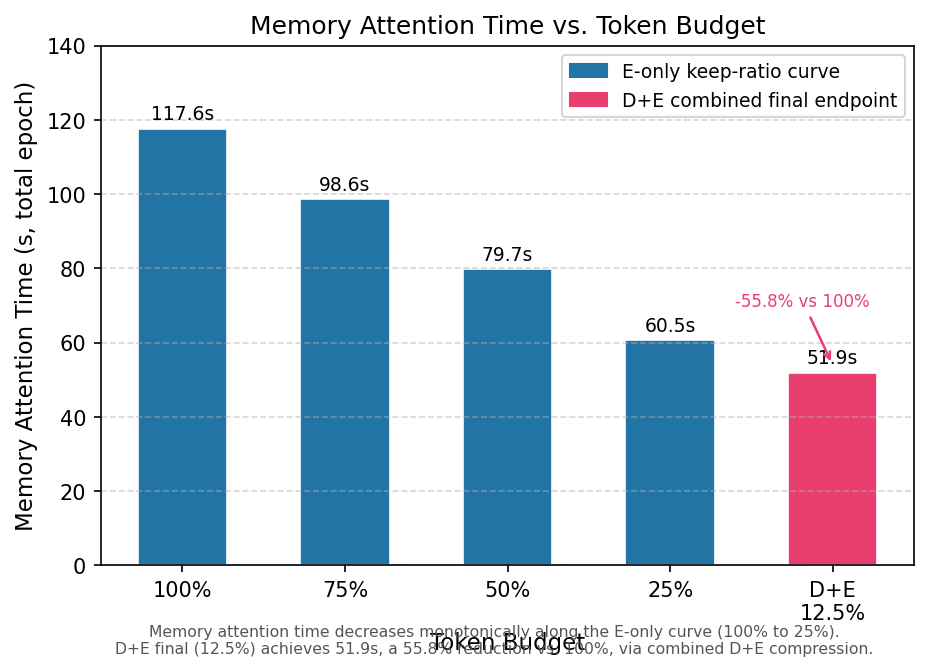
\includegraphics[width=0.78\linewidth]{figures/fig_token_budget_attention_time.png}
    \caption{Relationship between Token Budget and Memory Attention Time under fixed pseudo-label ablation setting. 100\%--25\% is the curve using only SMR, with 12.5\% being the MTC+SMR combination endpoint.}
    \label{fig:token_budget_attention}
\end{figure}

\subsection{Auxiliary PQR Ablation}
\begin{table}[t]
  \centering
  \small
  \setlength{\tabcolsep}{4pt}
  \renewcommand{\arraystretch}{1.08}
  \caption{Auxiliary pseudo-label quality ablation under fixed pseudo-label setting. Results only used to explore supervision reliability, not constituting main performance conclusions of this paper.}
  \label{tab:pseudo_label_ablation}
  \begin{tabular}{lccc}
    \toprule
    Method & mIoU$\uparrow$ & vs. R0 & vs. Previous \\
    \midrule
    Identity (R0) & 60.02 & -- & -- \\
    Class-balanced Filtering (R2) & 60.07 & +0.05 & +0.05 \\
    + Prototype-guided Gating (R2+R4) & 60.05 & +0.03 & -0.02 \\
    \bottomrule
  \end{tabular}
\end{table}


In Table~\ref{tab:pseudo_label_ablation}, mIoU for Identity, class-balanced filtering, and prototype-guided gating are 60.02, 60.07, and 60.05, respectively. Class-balanced filtering only brings $+0.05$, indicating that adjusting class coverage may slightly improve target domain supervision, but the change magnitude is insufficient to support strong conclusions; adding prototype gating does not further improve. One possible reason is that additional filtering reduces effective supervision, or batch-level prototypes remain unstable for rare classes and domain shift. Since these interpretations have not yet been verified by more diagnostics, PQR serves only as auxiliary exploration of pseudo-label reliability and does not constitute the main contribution.

Synthesizing ablation results, MTC+SMR has the most direct evidence for reducing memory attention overhead, but lower token budgets increase risks of fine-grained semantic and boundary losses. Module ablation explains the source of efficiency gains, token budget defines compression strength, and PQR only supplements supervision reliability analysis; the experimental roles of the three cannot be exchanged. Training efficiency and segmentation quality need to be jointly balanced.
